\documentclass[../handbook.tex]{subfiles}
\graphicspath{{\subfix{../pics/}}}
\begin{document}

\chapter{Boostrap}

Довольно мощный тест который позволяет вычислить параметры распределения или
какие-то дополнительные метрики по выборке.

Положим, что у нас какая-то \emph{репрезентативная} выборка~$S$ и мы хотим
оценить некоторый параметр~$\nu$. Например, это может быть первый квартиль или
разность матожиданий. 

Чтобы провести bootstrap проведем~$X(> 1000)$ раз процедуру:
\begin{enumerate}
    \item Просэмплируем из множества~$S$ подвыборку~$N$ элементов с возвращениями. На практике достаточно $50 < N < 100$.
    \item Посчитаем на полученной подвыборке параметр~$\nu$.
\end{enumerate}
В итоге мы получаем новую выборку из $X$ оценок параметра~$\nu$ и теперь можем оценить и как матожидание этого параметра, так и его доверительный интервал.

\emph{Дальше теория почему это работает.}

\section{Состоятельная оценка}

\marginpar{
    $X_1,\, \ldots,\, X_n \sim F_\theta$ --- случайная выборка \\
    $\theta \in \Theta$ --- параметр распределения~$F$ \\
    $\hat \theta = \hat\theta(X_1,\,\ldots,\,X_n)$ --- оценка параметра~$\theta$
}
Оценка~$\hat\theta$ называется \emph{состоятельной} если есть сходимость по вероятности
\begin{equation}
    \label{eq:consisten_estimator}
    \hat\theta \xrightarrow[n \to \infty]{\mathbb{P}} \theta 
\end{equation}

Другими словами, чем больше мы будем проводить наблюдений, тем более точно мы сможем оценить параметр~$\theta$.

\section{Эмпирическое распределение}

Предположим, мы хотим восстановить неизвестное распределение~$F$ по выборке~$X = (X_1,\,\ldots,\,X_n)$. Создадим оценку функции распределения таким образом

\begin{equation}
    \label{eq:emirical_cdf}
    \hat F_n(y) = \frac1n \sum_{i=1}^n \mathbb{I}(X_i < y)
\end{equation}

\begin{marginfigure}
    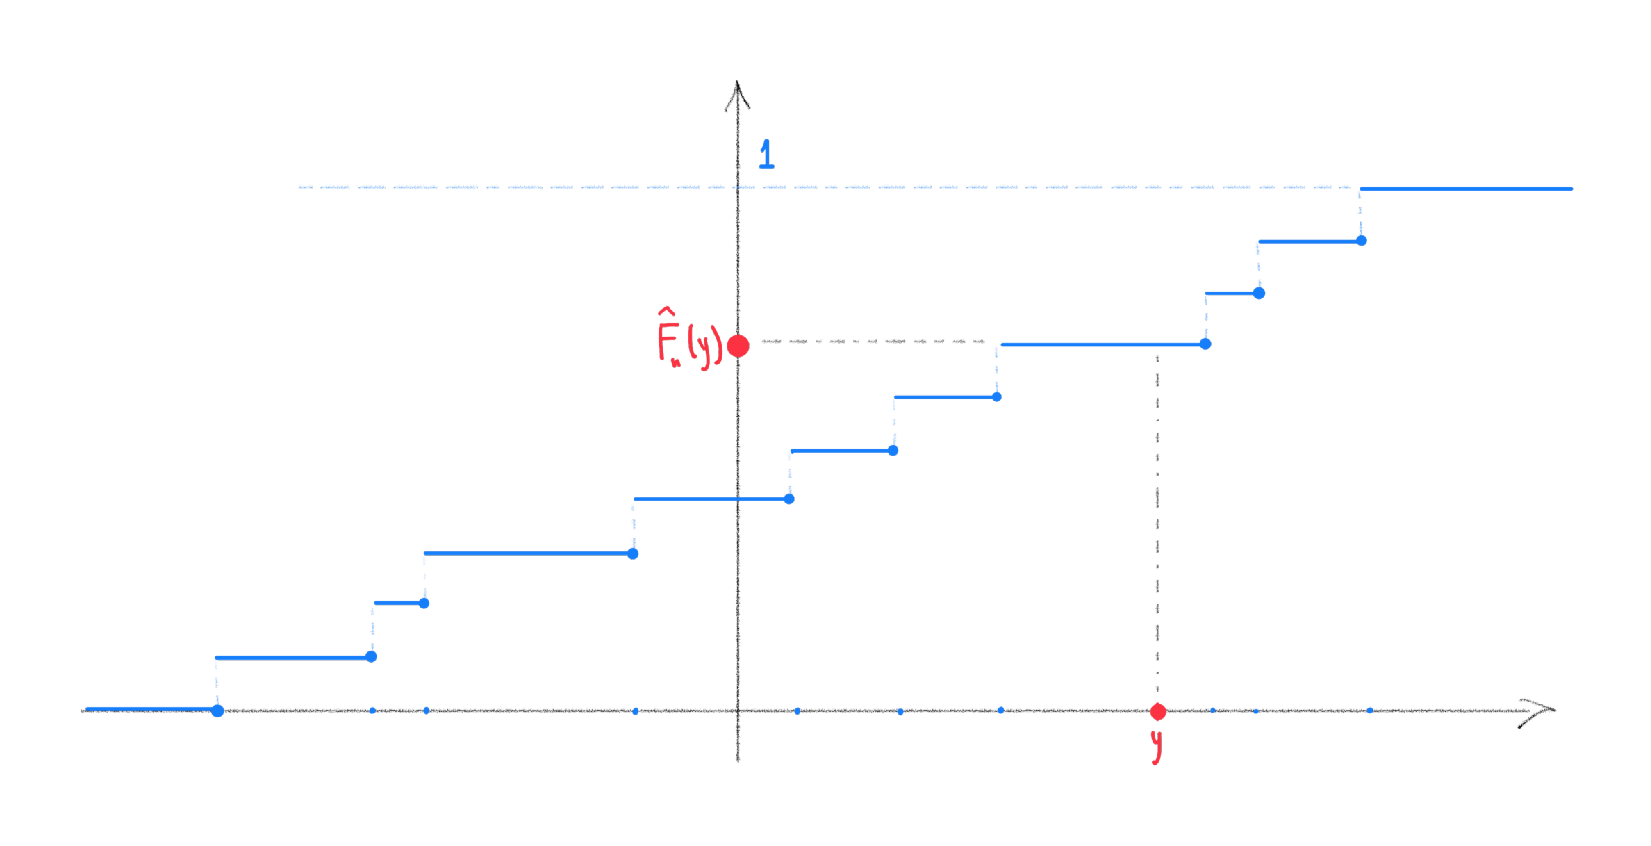
\includegraphics[width=1\columnwidth]{empirical_distr.pdf}
    \label{fig:empirical_distr}
\end{marginfigure}

\begin{theorem}
    Если~$M(F) < \infty$, тогда для любого~$y\in\mathbb{R}$ оценка $\hat F_n(y)$ состоятельна, то есть
    \begin{equation}
        \label{eq:emp_cdf_theorem}
        \hat F_n(y) \xrightarrow[n \to \infty]{\mathbb{P}} F(y)%, \qquad \text{для любого~}y
    \end{equation}
\end{theorem}
\sidenote{\fullcite{cher2003_lectures}}
\begin{proof}
    Случайные величины $\mathbb I(X_i < y)$ независимы и одинаково распределены, тогда достаточно оценить мат.ожидание только для~$\mathbb I(X_1 < y)$.

    \[
        M\,\mathbb I(X_1 < y) = 1 \cdot P(X_1 < y) + 0 \cdot P(X_1 \geq y) = P(X_1 < y) = F(y) < \infty.
    \]
По ЗБЧ Хинчина~\ref{sec:low_of_large_number}
\[
    \hat F_n(y) =
        \frac{\sum_{i=1}^n \mathbb{I}(X_i < y)}{n} 
        \xrightarrow[n \to \infty]{\mathbb{P}}
    M\,\mathbb I(X_1 < y)
    = F(y)
\]
\end{proof}





\end{document}
